%\documentclass[conference]{IEEEtran}
\documentclass[11pt,letterpaper]{article}
\usepackage[margin=1in]{geometry}

\usepackage{cite}


\usepackage[bookmarks=true,pdfstartview=FitH,colorlinks,linkcolor=darkred,filecolor=darkred,citecolor=darkred,urlcolor=darkred]{hyperref}

\hyphenation{op-tical net-works semi-conduc-tor}

\usepackage{colortbl}
\usepackage{mdframed}
\usepackage{color,soul}
%\usepackage{tabstackengine}

\usepackage{paralist}
\usepackage{pdfpages}
\usepackage{enumitem}
\usepackage{float}
\usepackage{booktabs}
\usepackage[override]{cmtt}
%\usepackage{titlesec}
\usepackage{color,xcolor}

%\usepackage{inconsolata,graphicx,color,eso-pic}
\usepackage{graphicx,color,eso-pic}

\usepackage[
	lambda,
	advantage,
	operators,
	sets,
	adversary,
	landau,
	probability,
	notions,
	logic,
	ff,
	mm,
	primitives,
	events,
	complexity,
	asymptotics,
	keys]
{cryptocode}

\usepackage{tikz}
\usetikzlibrary{fit, shapes, positioning, patterns, arrows,shadows}

\tikzset{
    master/.style={
        execute at end picture={
            \coordinate (lower right) at (current bounding box.south east);
            \coordinate (upper left) at (current bounding box.north west);
        }
    },
    slave/.style={
        execute at end picture={
            \pgfresetboundingbox
            \path (upper left) rectangle (lower right);
        }
    }
}

%\definecolor{lightgray}{rgb}{0.85, 0.85, 0.85}
\sethlcolor{lightgray}
%% Macros used in this paper


%\newcommand{\data}{{\ensuremath{\mathsf{data}}}\xspace}
%\newcommand{\wdata}{{\mathsf{wdata}}}
%\newcommand{\fetched}{{\mathsf{rdata}}}

\newcommand{\trnode}{\ensuremath{\mathcal{B}}\xspace}

\newcommand{\cpu}{CPU\xspace}
\newcommand{\cpus}{CPUs\xspace}

\newcommand{\mem}{{\ensuremath{\mathsf{mem}}}\xspace}
\newcommand{\add}{{\ensuremath{\mathsf{addr}}}\xspace}

\newcommand{\Read}{{\ensuremath{\mathsf{read}}}\xspace}
\newcommand{\Write}{{\ensuremath{\mathsf{write}}}\xspace}

\newcommand{\rf}{{\ensuremath{\mathsf{ref}}}\xspace}
\newcommand{\pos}{{\ensuremath{\mathsf{pos}}}\xspace}
\newcommand{\opram}{{\ensuremath{\mathsf{OPRAM}}}\xspace}
\newcommand{\PQ}{{\ensuremath{\mathsf{PQ}}}\xspace}
\newcommand{\PathOHeap}{{\ensuremath{\mathsf{PathOHeap}}}\xspace}
\newcommand{\PathOHeapinf}{{\ensuremath{\mathsf{PathOHeap}_{\infty}}}\xspace}
\newcommand{\PQinf}{{\ensuremath{\mathsf{PQ}_\infty}}\xspace}



\newcommand{\flag}{{\sf flag}\xspace}
\newcommand{\dummy}{{\sf dummy}\xspace}


\newcommand{\bfA}{\mathbf{A}}   \newcommand{\bfa}{\mathbf{a}}
\newcommand{\bfB}{\mathbf{B}}   \newcommand{\bfb}{\mathbf{b}}
\newcommand{\bfC}{\mathbf{C}}   \newcommand{\bfc}{\mathbf{c}}
\newcommand{\bfD}{\mathbf{D}}   \newcommand{\bfd}{\mathbf{d}}
\newcommand{\bfE}{\mathbf{E}}   \newcommand{\bfe}{\mathbf{e}}
\newcommand{\bfF}{\mathbf{F}}   \newcommand{\bff}{\mathbf{f}}
\newcommand{\bfG}{\mathbf{G}}   \newcommand{\bfg}{\mathbf{g}}
\newcommand{\bfH}{\mathbf{H}}   \newcommand{\bfh}{\mathbf{h}}
\newcommand{\bfI}{\mathbf{I}}   \newcommand{\bfi}{\mathbf{i}}
\newcommand{\bfK}{\mathbf{K}}   \newcommand{\bfk}{\mathbf{k}}
\newcommand{\bfL}{\mathbf{L}}   \newcommand{\bfl}{\mathbf{l}}
\newcommand{\bfM}{\mathbf{M}}   \newcommand{\bfm}{\mathbf{m}}
\newcommand{\bfN}{\mathbf{N}}   \newcommand{\bfn}{\mathbf{n}}
\newcommand{\bfO}{\mathbf{O}}   \newcommand{\bfo}{\mathbf{o}}
\newcommand{\bfP}{\mathbf{P}}   \newcommand{\bfp}{\mathbf{p}}
\newcommand{\bfQ}{\mathbf{Q}}   \newcommand{\bfq}{\mathbf{q}}
\newcommand{\bfR}{\mathbf{R}}   \newcommand{\bfr}{\mathbf{r}}
\newcommand{\bfS}{\mathbf{S}}   \newcommand{\bfs}{\mathbf{s}}
\newcommand{\bfT}{\mathbf{T}}   \newcommand{\bft}{\mathbf{t}}
\newcommand{\bfU}{\mathbf{U}}   \newcommand{\bfu}{\mathbf{u}}
\newcommand{\bfV}{\mathbf{V}}   \newcommand{\bfv}{\mathbf{v}}
\newcommand{\bfW}{\mathbf{W}}   \newcommand{\bfw}{\mathbf{w}}
\newcommand{\bfX}{\mathbf{X}}   \newcommand{\bfx}{\mathbf{x}}
\newcommand{\bfY}{\mathbf{Y}}   \newcommand{\bfy}{\mathbf{y}}
\newcommand{\bfZ}{\mathbf{Z}}   \newcommand{\bfz}{\mathbf{z}}

\newcommand{\nikhil}[1]{{\footnotesize\color{blue}[Nikhil: #1]}}





\renewcommand{\highlightkeyword}[2][\ ]{\ensuremath{\textrm{#2}}#1}

%\titlespacing{\section}{0pt}{*2.5}{*1.5}
%\titlespacing{\subsection}{0pt}{*2}{*0.8}
%\titlespacing{\subsubsection}{0pt}{*0.5}{*0}
%\newcommand{\ignore}[1]{}

\newcommand{\msf}[1]{\ensuremath{{\mathsf {#1}}}}
%\newcommand{\mtt}[1]{\ensuremath{\mathtt {#1}}}
\newcommand{\mcal}[1]{\ensuremath{\mathcal {#1}}}
\newcommand{\fsgx}{{\color{darkred}{\ensuremath{\mcal{G}_{\textrm{sgx}}}}}\xspace}
\newcommand{\ftpm}{{\color{darkred}{\ensuremath{\mcal{G}_{\textrm{tpm}}}}}\xspace}
\newcommand{\fsgxrelax}{{\color{darkred}{\ensuremath{\widetilde{\mcal{G}}_{\textrm{sgx}}}}}\xspace}
\newcommand{\ftpmrelax}{{\color{darkred}{\ensuremath{\widetilde{\mcal{G}}_{\textrm{tpm}}}}}\xspace}
\newcommand{\foutsource}{{\color{darkred}{\ensuremath{\mcal{F}_{\textrm{outsrc}}}}}\xspace}
\newcommand{\fenclave}{{\color{darkred}{\ensuremath{\mcal{F}_{\textrm{enclave}}}}}\xspace}
\newcommand{\fsc}{{\color{darkred}{\ensuremath{\mcal{F}_{\textrm{sc}}}}}\xspace}
\newcommand{\fauth}{{\color{darkred}{\ensuremath{\mcal{F}_{\textrm{auth}}}}}\xspace}
\newcommand{\fstatefulobf}{{\color{darkred}{\ensuremath{\mcal{F}_{\textrm{statefulobf}}}}}\xspace}
\newcommand{\fsgxprime}{{\color{darkred}{\ensuremath{\widehat{\mcal{G}}_{\textrm{sgx}}}}}\xspace}
\newcommand{\fcom}{{\color{darkred}{\ensuremath{\mcal{F}_{\textrm{com}}}}}\xspace}
\newcommand{\ftwopc}{{\color{darkred}{\ensuremath{\mcal{F}_{\textrm{2pc}}}}}\xspace}
\newcommand{\fmpc}{{\color{darkred}{\ensuremath{\mcal{F}_{\textrm{mpc}}}}}\xspace}

\newcommand{\algM}{{\color{darkred}\ensuremath{\mcal{M}}}\xspace}
\newcommand{\algS}{{\color{black}\ensuremath{{\sf Sim}}}\xspace}
\newcommand{\algC}{{\color{black}\ensuremath{\mcal{C}}}\xspace}
\newcommand{\algP}{{\color{darkred}\ensuremath{\mcal{P}}}\xspace}
\newcommand{\algPi}{{\color{darkred}\ensuremath{\mcal{P}_i}}\xspace}
\newcommand{\algPj}{{\color{darkred}\ensuremath{\mcal{P}_j}}\xspace}
\newcommand{\algPone}{{\color{darkred}\ensuremath{\mcal{P}_1}}\xspace}
\newcommand{\algPn}{{\color{darkred}\ensuremath{\mcal{P}_n}}\xspace}
\newcommand{\algR}{{\color{darkred}\ensuremath{\mcal{R}}}\xspace}
\newcommand{\algA}{{\ensuremath{\mcal{A}}}\xspace}
\newcommand{\algB}{{\ensuremath{\mcal{B}}}\xspace}
\renewcommand{\adv}{{\color{black}\ensuremath{\mcal{A}}}\xspace}
\newcommand{\envi}{{\color{darkred}\ensuremath{{\mcal{Z}}}}\xspace}
\newcommand{\algZ}{{\color{darkred}\ensuremath{{\mcal{Z}}}}\xspace}
\newcommand{\Sim}{\ensuremath{\msf{Sim}}\xspace}
%\newcommand{\st}{\ensuremath{{\it st}}\xspace}

\newcommand{\ct}{\ensuremath{{\sf ct}}\xspace}
\newcommand{\CT}{\ensuremath{{\sf CT}}\xspace}
\renewcommand{\ppt}{\ensuremath{{\text{p.p.t.}}}\xspace}
\renewcommand{\poly}{\ensuremath{{{\sf poly}}}\xspace}
\newcommand{\type}{\ensuremath{{\sf type}}\xspace}
\newcommand{\authenc}{\ensuremath{{\sf AE}}}

\renewcommand{\TC}{\ensuremath{{\bf TC}}}
\newcommand{\LC}{\ensuremath{{\bf LC}}}
\newcommand{\req}{\ensuremath{{\sf req}}\xspace}
\renewcommand{\d}{\ensuremath{\mathfrak{\delta}}\xspace}
\newcommand{\tc}{\ensuremath{\mathrm{tc}}}
\newcommand{\lc}{\ensuremath{\mathrm{lc}}}
\newcommand{\R}{\ensuremath{\mathbb{R}}}
\newcommand{\Alg}{\mathcal{A}}
%\newcommand{\dist}{\textrm{dist}}
\newcommand{\Fam}{\mathcal{F}}
\newcommand{\E}{\mathbb{E}}
\newcommand{\In}{\textrm{In}}
\newcommand{\eps}{\varepsilon}
\newcommand{\iseq}{\overset{\text{?}}{=}}

%\newcommand{\view}{\ensuremath{{\sf view}}\xspace}

\newcommand{\ie}{i.e.,\xspace}
\newcommand{\eg}{e.g.,\xspace}
\newcommand{\mcfe}{{\ensuremath{\sf MCFE}}\xspace}
\newcommand{\mcfeffh}{{\ensuremath{{\sf MCFE}^{\rm ffh}}}\xspace}
\newcommand{\MCFEffh}{{\ensuremath{{\sf MCFE}^{\rm ffh}}}\xspace}
\newcommand{\MCIPE}{{\ensuremath{\sf MCFE}}\xspace}
\newcommand{\MCFE}{{\ensuremath{\sf MCFE}}\xspace}
\newcommand{\FE}{{\ensuremath{\sf FE}}\xspace}
\newcommand{\fe}{{\ensuremath{\sf FE}}\xspace}
\newcommand{\SE}{{\ensuremath{\sf SE}}\xspace}
\newcommand{\Leak}{{\ensuremath{\sf Leak}}\xspace}
\newcommand{\HH}{{\ensuremath{\sf HH}}\xspace}
\newcommand{\HHb}{{\ensuremath{{\sf HH}^b}}\xspace}
\newcommand{\HK}{{\ensuremath{\sf HK}}\xspace}
\newcommand{\HKb}{{\ensuremath{{\sf HK}^b}}\xspace}
%\newcommand{\HH}{\ensuremath{{\mcal{S}_{\rm HH}}}\xspace}
%\newcommand{\HHb}{\ensuremath{{\mcal{S}^b_{\rm HH}}}\xspace}
%\newcommand{\HK}{\ensuremath{{\mcal{S}_{\rm HK}}}\xspace}
%\newcommand{\HKb}{\ensuremath{{\mcal{S}^b_{\rm HK}}}\xspace}
%\newcommand{\HH}{{\ensuremath{\mcal{H}_S^{\rightarrow H}}}\xspace}
%\newcommand{\HK}{{\ensuremath{\sf HK}}\xspace}
%\newcommand{\HK}{{\ensuremath{\mcal{H}_S^{\rightarrow K}}}\xspace}
%\newcommand{\HK}{{\ensuremath{\sf HK}}\xspace}
\newcommand{\tPKE}{{\ensuremath{\sf tPKE}}\xspace}
\newcommand{\tpk}{{\ensuremath{\sf tpk}}\xspace}
\newcommand{\epk}{{\ensuremath{\sf epk}}\xspace}
\newcommand{\esk}{{\ensuremath{\sf esk}}\xspace}
\newcommand{\cprf}{{\ensuremath{\sf CPRF}}\xspace}
\newcommand{\online}{{\ensuremath{\mcal{O}}}\xspace}

\renewcommand{\iO}{\ensuremath{{{\sf iO}}}\xspace}
\newcommand{\io}{\ensuremath{{{\sf iO}}}\xspace}
\newcommand{\pio}{\ensuremath{{{\sf piO}}}\xspace}
\newcommand{\piO}{\ensuremath{{{\sf piO}}}\xspace}


\newcommand{\param}{\ensuremath{{\sf pp}}\xspace}
\newcommand{\Gen}{\ensuremath{{\bf Gen}}\xspace}
\newcommand{\Setup}{\ensuremath{{\bf Setup}}\xspace}
\newcommand{\Expt}{\ensuremath{{\sf Expt}}\xspace}
\newcommand{\Real}{\ensuremath{{\sf Real}}\xspace}
\newcommand{\Ideal}{\ensuremath{{\sf Ideal}}\xspace}
\newcommand{\Hyb}{\ensuremath{{\sf Hyb}}\xspace}
\newcommand{\Gb}{\ensuremath{{\bf Gb}}\xspace}
\newcommand{\Eval}{\ensuremath{{\bf Eval}}\xspace}
\newcommand{\Enc}{\ensuremath{{\bf Enc}}\xspace}
\newcommand{\Rte}{\ensuremath{{\bf Rte}}\xspace}
\newcommand{\Dec}{\ensuremath{{\bf Dec}}\xspace}
\newcommand{\KeyGen}{\ensuremath{{\bf KGen}}\xspace}
\newcommand{\KGen}{\ensuremath{{\bf KGen}}\xspace}
\renewcommand{\prf}{\ensuremath{{\sf PRF}}\xspace}
\newcommand{\PRF}{\ensuremath{{\sf PRF}}\xspace}
\newcommand{\boldtau}{\ensuremath{{\boldsymbol{\tau}}}\xspace}


\newcommand{\ek}{\ensuremath{{\sf ek}}\xspace}
\newcommand{\gsk}{\ensuremath{{\sf gsk}}\xspace}
\newcommand{\dk}{\ensuremath{{\sf dk}}\xspace}
\newcommand{\rk}{\ensuremath{{\sf rk}}\xspace}
\newcommand{\tk}{\ensuremath{{\sf tk}}\xspace}
\newcommand{\crupt}{\ensuremath{{\sf crupt}}\xspace}
%\newcommand{\ct}{\ensuremath{{\bf ct}}\xspace}





\newcommand{\TODO}[1]{\noindent
\colorbox{green!20}{
\parbox{0.98\textwidth}{
#1
}}
}

\definecolor{darkgreen}{rgb}{0,0.5,0}
\definecolor{lightblue}{RGB}{0,176,240}
\definecolor{darkblue}{RGB}{0,112,192}
\definecolor{lightpurple}{RGB}{124, 66, 168}
%\definecolor{orange}{rgb}{1,0.5,0}
\definecolor{grey}{RGB}{139, 137, 137}
\definecolor{maroon}{RGB}{178, 34, 34}
\definecolor{green}{RGB}{34, 139, 34}
\definecolor{types}{RGB}{72, 61, 139}
%\definecolor{gold}{rgb}{0.85, 0.65, 0.13}
\definecolor{gold}{rgb}{0.8, 0.33, 0.0}

\newcommand{\sred}[1]{{\color{maroon} \msf{#1}}}
\newcommand{\sblue}[1]{{\color{lightblue} {#1}}}
\newcommand{\spurple}[1]{{\color{lightpurple} \msf{#1}}}
\newcommand{\sorange}[1]{{\color{orange} \msf{#1}}}
\newcommand{\sgold}[1]{{\color{gold} {#1}}}
\newcommand{\smaroon}[1]{{\color{maroon} {#1}}}
\newcommand{\sgrey}[1]{{\color{grey} \msf{#1}}}
\newcommand{\sseablue}[1]{{\color{darkblue} {\bf #1}}}
\newcommand{\sdarkgreen}[1]{{\color{darkgreen} {#1}}}
\newcommand{\sdarkblue}[1]{{\color{darkblue} {#1}}}

\definecolor{darkgray}{gray}{0.3}
\newcommand{\cgray}[1]{{\color{darkgray} {#1}}}
\newcommand{\sgray}[1]{{\color{gray!100} {#1}}}
\newcommand{\skiptext}[1]{}
%\newcommand{\envi}{\ensuremath{{\sf env}}\xspace}
\newcommand{\msg}{\ensuremath{{{\sf msg}}}\xspace}
%\newcommand{\owf}{\ensuremath{{{\sf owf}}}\xspace}
\newcommand{\comm}{\ensuremath{{{\sf com}}}\xspace}
\newcommand{\mpc}{\ensuremath{{{\sf mpc}}}\xspace}
\newcommand{\getr}{\ensuremath{{\overset{\$}{\leftarrow}}}\xspace}
\renewcommand{\sample}{\ensuremath{{\overset{\$}{\leftarrow}}}\xspace}
\newcommand{\some}{{some \xspace}}

\newcommand{\Prot}{\ensuremath{{{\bf Prot}}}\xspace}

\newcommand{\install}{{\color{darkblue} \ensuremath{{{\tt install}}}\xspace}}
\newcommand{\resume}{{\color{darkblue} \ensuremath{{{\tt resume}}}\xspace}}
\newcommand{\getpk}{{\color{darkblue} \ensuremath{{{\tt getpk}}}\xspace}}
\newcommand{\corrupt}{{\color{darkblue} \ensuremath{{{\tt corrupt}}}\xspace}}
%\newcommand{\sign}{{\color{darkblue} \ensuremath{{{\tt sign}}}\xspace}}

\newcommand{\mpk}{\ensuremath{{\sf mpk}}\xspace}
\newcommand{\msk}{\ensuremath{{\sf msk}}\xspace}
\newcommand{\RO}{\ensuremath{{\sf RO}}\xspace}



%%%
%%% FAN's MACRO 
%%% XXX
%%%
\newcommand{\onrcv}{\xspace\sblue{On~receive}\xspace}
\newcommand{\oninp}{\xspace\sblue{On~input}\xspace}
\newcommand{\oncall}{\xspace\sblue{On~call}\xspace}

\newcommand{\onrcvonce}{\xspace\sdarkgreen{On~receive}\xspace}
\newcommand{\oninponce}{\xspace\sdarkgreen{On~input}\xspace}
\newcommand{\pcforall}{{\bf for all}\xspace}
%\renewcommand{\pcreturn}{output\xspace}
%\renewcommand{\pcif}{if\xspace}
%\renewcommand{\pcelse}{else\xspace}
%\renewcommand{\pcfor}{for\xspace}
%\renewcommand{\pcthen}{then\xspace}

\newcommand{\progcomment}[1]{\cgray{\small \it //~#1}}

% vars
\newcommand{\inpfsgx}{{\ensuremath{{{\color{black}\sf inp}}}}}
\newcommand{\inp}{{\ensuremath{{{\color{black}\sf inp}}}}}
\newcommand{\outpfsgx}{{\ensuremath{{{\color{black}\sf outp}}}}}
\newcommand{\outp}{{\ensuremath{{{\color{black}\sf outp}}}}}
\newcommand{\regfsgx}{{\ensuremath{{{\color{black}\sf reg}}}}}

% keywords
\newcommand{\memfsgx}{{\ensuremath{\sf{{\color{black}mem}}}}}
\newcommand{\prog}{{\ensuremath{\sf{{\color{black}prog}}}}}
\newcommand{\progfsgx}{{\ensuremath{\sf{{\color{black}prog}}}}}
\newcommand{\iffsgx}{{\xspace{{\color{black}if}}\xspace}}

% operations
\newcommand{\assertfsgx}{{assert}\xspace}
\newcommand{\recordfsgx}{{record}\xspace}
\newcommand{\sendfsgx}{{\color{darkblue}{asend}}\xspace}
\newcommand{\secsendfsgx}{{\color{darkblue}{ssend}}\xspace}
\newcommand{\letfsgx}{{let}\xspace}
\newcommand{\returnfsgx}{{return}\xspace}

% strings
\newcommand{\stringfsgx}[1]{{\color{brown}\textrm{``{#1}''}}}
\newcommand{\party}[1]{{{\color{darkred}#1}}\xspace}
\newcommand{\func}[1]{\ensuremath{{\color{darkred}\mcal{#1}}}\xspace}

% lineno
\newcommand{\lnn}[1]{\small{\texttt{#1}}\xspace}



\newcommand{\appendices}{appendices\xspace}



\usepackage{boxedminipage}
%\usepackage{fancyhdr}
%\usepackage{djb}
\usepackage{cite}
%\usepackage{times}
%\usepackage{array}
\usepackage{url}
%\usepackage{pdfpages}
%\usepackage{listings}
%\usepackage{fullpage}
%\usepackage[left=1in,top=1in,right=1in,bottom=1in]{geometry}
%\usepackage{graphics}
%\usepackage{graphicx,proof}
\usepackage{graphicx}
%\usepackage{algorithm2e}
\usepackage[bf,justification=centering]{caption}
\usepackage[justification=centering]{subcaption}
%\usepackage{subcaption}
%\usepackage{epsfig,psfrag}
\usepackage{color}
%\usepackage{comment}
\usepackage{xspace}
\usepackage{multirow}
%\usepackage[sort&compress,sectionbib]{natbib}

\usepackage{amsthm}
%\usepackage{fdsymbol}
%\undef\centerdot
%\undef\circledS
%\undef\thicksim
%\undef\thickapprox
%\undef\hslash


%\usepackage{amsthm,amstext}
\usepackage{amsmath,amsthm,amstext,amsfonts,amssymb,latexsym}
\usepackage{amsbsy}
\usepackage{stmaryrd}
\usepackage{pifont}

\setcounter{MaxMatrixCols}{15}

\newcommand\smallblacktriangledown{%
   \vcenter{\hbox{${\scriptscriptstyle\blacktriangledown}$}}}
\newcommand\smalltriangledown{%
   \vcenter{\hbox{${\scriptscriptstyle\triangledown}$}}}
\newcommand{\piinv}{\ensuremath{\pi^{{\scriptscriptstyle{-}}1}}\xspace}


\newcommand\whitestar{{\ensuremath{\mbox{\scriptsize \ding{65}}}}\xspace}

%\renewcommand{\widehat}{\mathaccent "0670\relax}
%\renewcommand{\widetilde}{\mathaccent "0672\relax}


%\usepackage{amsmath,amsthm,amstext,amsfonts,latexsym}
%\usepackage{shortcuts}
%\usepackage{code}
\usepackage{wrapfig}


\usepackage{algorithm}
\usepackage[noend]{algpseudocode}
\usepackage{algorithmicx}

%\usepackage{algorithm2e}



%\setlength{\floatsep}{0.5ex}
%\setlength{\textfloatsep}{3pt}
%\setlength{\abovecaptionskip}{3pt}
%\setlength{\belowcaptionskip}{0ex}

%\setlength{\parsep}{0pt}

%\pagestyle{fancy}
%\headheight 35pt

\definecolor{darkred}{rgb}{0.5, 0, 0}
\definecolor{darkgreen}{rgb}{0, 0.5, 0}
\definecolor{darkblue}{rgb}{0,0,0.5}


%\lhead{\thepage \quad \quad \quad Ensighta Security Inc.}
%\rhead{Topic \# A10-013 \quad Proposal \# Army SBIR 2010.1}
%\lhead{\thepage}
%\chead{}
%\fancyfoot{}
%\chead{Ensighta Security Inc.}
%\setpagewiselinenumbers
%\linenumbers
%\pagewiselinenumbers

%\setlength{\textwidth}{7in} \setlength{\textheight}{9.62in}

{
\theoremstyle{definition}
\newtheorem{definition}{Definition}
}
%\newtheorem{proposition}{Proposition}
%\newtheorem{example}{Example}

%\usepackage{breakurl}
%\def\baselinestretch{0.97}
% center the one-line caption of a figure.
%\centerfigcaptionstrue
%\newcommand\markx[2]{\mbox{}\marginpar{\raggedright\hspace{0pt}#1:#2}}
\newcommand\markx[2]{}
\newcommand\markme[1]{\markx{ME}{#1}}
\newcommand\markjim[1]{\markx{JIM}{#1}}
\newcommand\marka[1]{\markx{R1}{#1}}
\newcommand\markb[1]{\markx{R2}{#1}}
\newcommand\markc[1]{\markx{R3}{#1}}

\newcommand{\marknew}{}
\newcommand{\DB}{\mathbf{DB}}


%\newcommand{\model}{\mathbf{\Omega}}
%\newcommand{\appendices}{supplementary materials\xspace}

%\newcommand{\authnote}[2]{{\bf #1 : #2}}
%\newcommand{\authnote}[2]{}

\newcommand{\david}[1]{{\authnote{david}{#1}}}
%\newcommand{\runting}[1]{{\authnote{runting}{#1}}}
\newcommand{\runting}[1]{{\footnotesize\color{red}[runting: #1]}}
\newcommand{\futureresearch}[1]{{\footnotesize\color{red}[dawn: #1]}}
\newcommand{\jim}[1]{{\authnote{jim}{#1}}}
%\newcommand{\dawn}[1]{{\authnote{dawn}{#1}}}
\newcommand{\zk}[1]{{\authnote{zk}{#1}}}
\newcommand{\cody}[1]{{\authnote{cody}{#1}}}
\newcommand{\heng}[1]{{\authnote{heng}{#1}}}
\newcommand{\name}{Circuit OPRAM\xspace}
%\newcommand{\aname}{an Elixir\xspace}
%\newcommand{\Aname}{An Elixir\xspace}

\newcommand{\pid}{{\color{darkgray}\mathit{pid}}}
\newcommand{\idx}{{\color{darkgray}\mathit{idx}}}
\newcommand{\eid}{{\color{darkgray}\mathit{eid}}}
\newcommand{\sid}{{\color{darkgray}\mathit{sid}}}
\newcommand{\ssid}{{\color{darkgray}\mathit{ssid}}}
%\newcommand{\sk}{\mathsf{sk}}
%\newcommand{\pk}{\mathsf{pk}}
%\newcommand{\idx}{\mathit{idx}}
%\newcommand{\poly}{\mathit{poly}}
\newcommand{\pc}{{\tt pc}}
\newcommand{\op}{\ensuremath{\mathsf{op}}\xspace}
\newcommand{\reg}{{\tt reg}}
\newcommand{\regs}{{\tt regs}}
\newcommand{\raddr}{{\tt raddr}}
\newcommand{\waddr}{{\tt waddr}}


\renewcommand{\path}{\ensuremath{\mathsf{path}}\xspace}
\newcommand{\block}{{\sf B}}


\newcommand{\src}{{\sf src}}
\newcommand{\dst}{{\sf dst}}



\newcommand{\Path}{{\sf path}}
\newcommand{\posmap}{{\sf posmap}}
\newcommand{\dataopram}{\ensuremath{{\sf data}\text{-}{\sf OPRAM}}\xspace}
\newcommand{\posopram}{\ensuremath{{\sf pos}\text{-}{\sf OPRAM}}\xspace}
\newcommand{\posoprams}{\ensuremath{{\sf pos}\text{-}{\sf OPRAM}\text{s}}\xspace}
%\newcommand{\root}{{\sf root}}


\newcommand{\data}{{\ensuremath{\mathsf{data}}}\xspace}
\newcommand{\addr}{{\ensuremath{\mathsf{addr}}}\xspace}
\newcommand{\phaddr}{{\ensuremath{\mathsf{phaddr}}}\xspace}
\newcommand{\fetched}{{\ensuremath{\mathsf{fetched}}}\xspace}
\newcommand{\wdata}{{\tt wdata}}
\newcommand{\rdata}{{\tt rdata}}
\newcommand{\OPRAM}{{\sf OPRAM}}
\newcommand{\rlvl}{d}
\newcommand{\RLVL}{D}
\newcommand{\rpos}{{\sf rpos}}
\newcommand{\lpos}{{\sf lpos}}
\newcommand{\aux}{{\sf aux}}
\newcommand{\elem}{{\sf elem}}
\newcommand{\pair}{{\sf pair}}
\newcommand{\used}{{\beta}}
\newcommand{\arr}{{\sf arr}}
\renewcommand{\negl}{{\sf negl}}
\newcommand{\reqs}{{\sf reqs}}
%\newcommand{\bLeft}{{\sf b}_0}
%\newcommand{\bRight}{{\sf b}_1}


\newcommand{\grp}[1]{{\ensuremath{\llbracket #1 \rrbracket}}\xspace}
\newcommand{\biggrp}[1]{\ensuremath{\left\llbracket #1 \right\rrbracket}\xspace}
\newcommand{\N}{\ensuremath{\mathbb{N}}\xspace}
\newcommand{\G}{\ensuremath{\mathbb{G}}\xspace}
\newcommand{\Z}{\ensuremath{\mathbb{Z}}\xspace}
\newcommand{\bfalpha}{\ensuremath{{\boldsymbol \alpha}}\xspace}
%\newcommand{\bfI}{\ensuremath{{\bf I}}\xspace}
%\newcommand{\bfC}{\ensuremath{{\bf C}}\xspace}
%\newcommand{\bfP}{\ensuremath{{\bf P}}\xspace}
%\newcommand{\bfM}{\ensuremath{{\bf M}\xspace}
\newcommand{\treesmall}{\ensuremath{{\tt tree}_{\blacktriangledown}}}
\newcommand{\treebig}{\ensuremath{{\tt tree}_{\clubsuit}}}

\newcommand{\SEE}{SEE\xspace}
\newcommand{\aSEE}{a SEE\xspace}
\newcommand{\ignore}[1]{}
\newcommand{\etal}{\textit{et al.}\xspace}

%\renewcommand{\paragraph}[1]{\vspace{6pt}\noindent\textbf{#1}}
\newcommand{\mypara}[1]{\vspace{10pt}\noindent\textbf{#1}}
\newcommand{\squish}{
      \setlength{\topsep}{0pt}
      \setlength{\itemsep}{0ex}
      \vspace{-1ex}
      \setlength{\parskip}{0pt}}


\newcommand{\pksgx}{\ensuremath{{\sf pk}_{\textrm{sgx}}}}
\newcommand{\sksgx}{\ensuremath{{\sf sk}_{\textrm{sgx}}}}
\newcommand{\user}{\ensuremath{{\sf U}}}



\newcounter{task}
\newenvironment{task}[1]{ \refstepcounter{task} \paragraph{Task T\arabic{task}: #1}}{}


\newenvironment{proofof}[1]{\noindent \textbf{Proof of #1:}}{\hfill \qed}


\newtheorem{thm}{Theorem}[section]      % A counter for Algorithms etc


\newtheorem{theorem}[thm]{Theorem}
\newtheorem{conj}[thm]{Conjecture}
\newtheorem{conjecture}[thm]{Conjecture}
\newtheorem{lemma}[thm]{Lemma}
\newtheorem*{lemma*}{Lemma}
\newtheorem{claim}[thm]{Claim}
\newtheorem{corollary}[thm]{Corollary}
\newtheorem{fact}[thm]{Fact}
\newtheorem{proposition}[thm]{Proposition}
%\newtheorem{example}[thm]{Example}



\newtheoremstyle{boxes}% name  
{2pt}% ?Space above ? 
{0pt}% ?Space below ?
{}% ?Body font ?
{}% ?Indent amount ?
{\bfseries}% ?Theorem head font?
{}% ?Punctuation after theorem head ?
{\newline}% ?Space after theorem head ?
{\thmname{#1}\thmnumber{ #2}:  
\thmnote{#3}}

\theoremstyle{boxes}
\newtheorem{myalgo}[thm]{Algorithm}%{\bf}{} %
\newtheorem{myfunc}[thm]{Functionality}%{\bf}{} %
\newtheorem{myconst}[thm]{Construction}%{\bf}{} %
%\newtheorem{algorithm}{Algorithm}

{
\theoremstyle{definition}
\newtheorem{remark}{Remark}
}

\newcommand{\elaine}[1]{{\footnotesize\color{magenta}[Elaine: #1]}}
\newcommand{\Hao}[1]{{\footnotesize\color{blue}[Hao: #1]}}
\renewcommand{\elaine}[1]{}
 \renewcommand{\Hao}[1]{}


\newcommand{\reactively}{}
\newcommand{\Reactively}{}
\newcommand{\reactive}{}
\newcommand{\Reactive}{}
\newcommand{\Rft}{Fault-tolerant\xspace}

\newenvironment{MyEnumerate}[1]{\begin{enumerate}\setlength{\itemsep}{0.1cm}
\setlength{\parskip}{-0.05cm} #1}{\end{enumerate}}
\newenvironment{MyItemize}[1]{\begin{itemize}\setlength{\itemsep}{0.1cm}
\setlength{\parskip}{-0.05cm} #1}{\end{itemize}}



\newcounter{cnt:challenge}

%\urlstyle{sf}

\newcommand{\elainetodo}[1]{%
    \colorbox{red!20}{%
\parbox{\textwidth}{
elaine: \\
 #1
    }
}
}

\newenvironment{solution}[1][\unskip]{%
\par
\noindent
\textbf{Solution #1:}
\noindent}
{}

\newif\ifhidesolutions
%\hidesolutionstrue %uncomment to hide solutions

\ifhidesolutions
\usepackage{environ}
\NewEnviron{hide}{}
\let\solution\hide
\let\endsolution\endhide
\fi

\newcommand{\rb}[1]{\colorbox{blue!20}{#1}}
\newcommand{\wt}[1]{{#1}}
\newcommand{\highlight}[1]{\colorbox{lightgray}{$\displaystyle #1$}}



%\pagecolor{black}
%\color{white}

\begin{document}
%
\title{{\bf Foundations of Blockchains - Consensus Lab}  \\
{\large {\bf Open Source Version}}
}
\author{}
\date{}

\maketitle



%{\Huge TODO: update the points and Submission instructions}
The lab is an open-source version of the Consensus Lab used in the Foundations of Blockchains course at Carnegie Mellon University. This version includes lab instructions, starter code, and setup instructions for the auto-grader using Gradescope.

\paragraph{Students} %your solution should be in PDF format.
For students, the content in this repository is sufficient for learning and practicing distributed consensus. You can test your code with the provided test cases in the "Test" folder. Your working file would be:

\begin{itemize}
    \item
          Checkpoint 0: \texttt{Majority\_Vote\_Adversary.java}
    \item
          Checkpoint 1: \texttt{Student\_Player.java}
    \item
          Checkpoint 2: \texttt{Dolev\_Strong\_FRound\_Adversary.java}
\end{itemize}

\paragraph{Instructors:}For instructors interested in using this lab in their course, please contact Junxi Song at 20001218sjx@gmail.com for the solution and additional test cases. In our current autograder setup, each checkpoint has test cases assigned point values:

\begin{itemize}
    \item
          Checkpoint 0: 16 test cases, each worth 1 point
    \item
          Checkpoint 1: 41 test cases, each worth 1 point
    \item
          Checkpoint 2: 12 test cases, each worth 1 point
\end{itemize}




%\paragraph{\Large Submission instructions.}


%>>>>>>> 415186ab36f55f7954ddae2f11267928b2ccd3e5

\pagebreak

\section{Introduction}
\label{sec:intro}
%Consensus mechanisms are pervasive. They allow distributed systems to agree on a joint view of the computation and make consistent decisions, allowing them to work together securely. Even before cryptocurrencies, which typically come to mind when thinking of consensus protocols, became popular, consensus mechanisms were widely used. In aircraft systems consensus protocols were used as early as 1970s in order to ensure that the aircraft control system can withstand a failure of one of its components.
In this lab, you will learn how to construct and analyze consensus protocols. In particular, we will start by implementing a toy ``majority vote'' protocol and understand why this protocol is insecure by designing attacks that violate the security properties (validity and consistency) of a consensus protocol. We will then implement the Dolev-Strong protocol, which is indeed a secure consensus mechanism. We will try understand why the Dolev-Strong protocol is designed exactly the way it is, and why certain variations and simplifications of it would break the protocol's security. To do this, you will be asked to design attacks that violate the consistency or the validity properties of insecure variants of Dolev-Strong.

%\input{Introduction}
\section{Project Structure}

% \begin{wrapfigure}{l}{0.382\textwidth}
%     \centering
%     \includegraphics[width=0.382\textwidth]{handout/project_structure.png}
% \end{wrapfigure}
\paragraph{\large Starter code.}
The starter code is in the folder {\tt Code}. All the code for Checkpoint 0, 1, and 2, including the project dependency and submission files, are included in this zip file.
%The handout for Checkpoint 2 is this as well and all 
%the details for it can be found in Section~\ref{sec:cp2}.



%After the releasing of Checkpoint 2, there will be another file uploaded to the folder. Read the ``Introduction'' section and 
%the ``Project Structure'' section to understand the framework.
%=======
%Read the Section~\ref{sec:intro} Introduction and Section~\ref{sec:structure} Project Structure to understand the framework.
%Download the starter code from \href{https://drive.google.com/drive/folders/1AE_SZClkbaKC8PFtOMcnd6aCjgOH-MTA?usp=sharing}{google drive here}. 
%All the code for Checkpoint 0 and 1, including the project dependency and submission files, are in the folder \texttt{Code}. 
%The Checkpoint 2 will be released on October 25. This release would involve a new version of \texttt{Dolev\_Strong\_Player.java} file that will be uploaded to the same google drive folder above. 

\paragraph{Directory structure.}
The main directory for the source code is
\begin{center}
    \texttt{code/src},
\end{center}
\noindent henceforth we also refer to this directory as {\tt ./}.
There are four folders under {\tt ./}.
\begin{enumerate}[leftmargin=5mm]
    \item
    The {\tt ./Main} folder has two factory for the list of adversaries and players in this project.
    \item
          The {\tt ./Protocol} folder has all protocols and their corresponding adversaries we provided to you, everything you need to change is in {\tt ./Protocol} folder,
    \item
          The {\tt ./Simulator} folder is the framework of the simulator, and
          we will explain what each class does shortly.
    \item Finally, the {\tt ./Test} folder contains some tests we have created for you.
          In our Autograder, we have additional hidden test cases,
          so we encourage you to write more adversaries and tests yourself.
\end{enumerate}


For each protocol or attack, we have created a file for you where your code should be,
you should complete your work without changing anything outside the designated file. To test your programs locally, you could run some tests we provided to you in the {\tt ./Test} folder.
%At the end of the project, you should be able to analyze basic consensus schemes and specifically understand the intuition behind the security properties achieved by such consensus protocols.


\subsection{Consensus Simulator Framework}
%\subsection{Engine, Signature, Authenticated Channel Model}

%The consensus simulator framework 
%has three main modules, idealized signature [Fsign], 
%authenticated channel [Fauth], and [simulation engine].
%\bigskip
The following modules in the consensus framework will be relevant to you.
Below, we explain them one by one.


%\paragraph{Signature module:}
\subsubsection{Idealized Signature Module}
%The idealized signature [Fsign] basically has two functions, 
% The idealized signature class {\tt Fsign} has two important functions:
% the {\tt sign} function signs a message on behalf of a player,
% the {\tt verification}
% function checks if
% a purported signature is valid given a message and a purported signer.

%sign a message for a player and check the signature. 
In your implementation, you can call the {\tt sign}
function in the {\tt Player} class (or any class that extends {\tt Player})
class to sign messages
on behalf of the player, and call
the {\tt verify}
function to verify if the purported signature is valid.

Specifically, {\tt Player.sign}
returns
a string that includes the message
itself, the signature,
and the signer.
This string is the {\tt json} serialization
of a {\tt SignedM} object
which we will explain shortly\footnote{If you are
    interested in JSON, you can learn more on how it works
    at \url{https://sites.google.com/site/gson/gson-user-guide}.
    %\href{https://sites.google.com/site/gson/gson-user-guide#TOC-Primitives-Examples}{here}.
}.


%that signs messages for you. 
%To sign a message, one could extend the {\tt Player} class and call the 
%{\tt sign} function there.   
%only verification method should be called in your implementation. 
%The {\tt verification} method takes the signer's id, the message, and the signature, then checks if  the purported signature is valid for the message given the signer. 
%this message is signed by the player under that signature. 
%\bigskip

%\noindent
%\textbf{Authenticated channel:}
\subsubsection{Authenticated Channel and Message Sending}

The communication between players is through an authenticated channel class
    {\tt Fauth}.
The channel is authenticated in the sense that the message
recipient can know who is the true sender.
To work with the authenticated channel, in your implementation, you
need to know that the messages that a player receives
is an object of the {\tt Package} class, which includes
the {\tt sender}, the {\tt receiver}, and the actual message {\tt strSignedM}
whose type is a raw {\tt String}.
It is guaranteed that the receiver identity agrees with the recipient's identity.

To parse the received string  {\tt strSignedM} (of type {\tt String}),
you can call
the {\tt Player.parseSingleMsg} function
(or call it from any object that extends {\tt Player})
to convert it to an object of the {\tt SignedM} class.
The {\tt SignedM} class
includes the actual message {\tt msg}  as a {\tt String},
the {\tt signer}, and the signature
    {\tt sig} as a {\tt String}.

To send a message, you can call
    {\tt Player.send}
which takes the message of the type {\tt String} to send,
and the recipient identity.
If you want the message
to be signed, you could directly pass
the output of {\tt Player.sign}
to {\tt Player.send}, since
    {\tt Player.sign}
is a wrapper that did all
the serialization work for you (as we explained earlier).




%The authenticated channel [Fauth] sends packages between players. The format of Packages sent by [Fauth] is string, and [Fauth] checks the identity of the sender by the private key. [Package] class is used for [Fauth] to record the sender, receiver, and message. [sender] in [Package] is the actual sender checked by the authenticated channel, while the signature (not in [Fauth]) is a mark used by the sender. In an unauthenticated channel, [sender] in [Package] may not be the real sender. 
%\bigskip

\subsubsection{Simulation Engine}
The simulation engine, i.e., the {\tt Simulation\_Engine}
class, will initialize
the idealized signature, the authenticated
channel, all players, as well as the provided adversary if any.
%Simulation engine will initialize the signature model, authenticated channel, all players, the provided adversary. To avoid framework attack, the simulator will assign each player a public id and a  private key corresponding to it. 
After the initialization, the simulator begins a round-by-round simulation.
In each round, the engine will call the {\tt action} method of each honest player and then call the adversary's {\tt attack} method.
There will be one global instance of the {\tt Simulation\_Engine}
class called {\tt engine}.
%Your code should not have to call {\tt engine} directly.
%If you want to check which round the player is in, you can call
%{\tt engine.roundNumber}.
Your code may need to call the following functions inside {\tt engine}:
\begin{itemize}[leftmargin=5mm]
    \item
          {\tt engine.roundNumber}:
          returns the current round number;
    \item
          {\tt engine.numOfPlayers}:
          returns the total number of players;
    \item
          {\tt engine.numOfFaultyPlayers}:
          returns the maximum number of faulty players.
    \item
          {\tt engine.checkOutput}:
          returns {\tt false} if either consistency or validity is broken during
          an execution of the protocol,
          else returns {\tt true}.

          %\item 
          %{\tt engine.numOfPlayers}:
\end{itemize}

%When you implemented a consensus player (which extends the {\tt Player} class), 
%you should call the 
%{\tt engine.output}
%when player wants to output an outcome.

%Simulation engine also has [terminate], [output], and [endRound] function which players should call if they want to terminate the protocol, output the final result, and end the current round.  
\ignore{
    \bigskip

    \subsection{Message Sending}
    In real world, the message sent by authenticated channels are not parsed and users need to parse the information themselves. Here we created the [Package] class and [SignedM] class to simulate the real world and help with parsing.
    \bigskip

    \noindent
    \textbf{Package:}

    We created a class [Package], used by the communication channel, which contains the message string, the sender, and the receiver, to tell the player what the message is, who the actual sender is, and who is this message for. However, player still needs to parse the message string to extract useful information.
    \bigskip

    \noindent
    \textbf{SignedM:}

    We created a class [SignedM] to help parse the signed messages. A signed message includes the actual message, which is the bit in the case of Dolev-Strong, the signer who signed this message, and the signature. We created a wrapper function to help with converting between [SignedM] object and the string used for [Package]. Read the documentation of the wrapper function if needed. If you're interested in JSON, you can learn more on how it works \href{https://sites.google.com/site/gson/gson-user-guide#TOC-Primitives-Examples}{here}.
}

\subsubsection{Adversary}
You will be asked to implement adversaries for some broken consensus protocols.
Your attack code will extend the {\tt Adversary} class.
    {\tt Adversary}.{\tt faulty\_players}
returns the list of
faulty players. The messages sent by faulty players are fully controlled
by the adversary.
The adversary can just call the faulty players' {\tt send} function
to send messages on their behalf.
The adversary has the capability of looking at what messages honest
players intend to send in the present round, before deciding
what messages the
faulty players want to send in this round.
To look at the honest messages of the present round,
you can call the {\tt Adversary}.{\tt honestMsgs}
function
which returns a list of {\tt Package}s.




\elaine{FILL}

\ignore{
    Adversary has two ways to attack, one is the delay of the messages, the second way is to control some faulty players and send messages to honest players. It can also see all messages sent by all players even before these messages are received.


    To preform the first way of attacking, the method $sendInThisRound$ decides which messages to send in the current round, while method $attack$ is called in each round by the simulation engine to perform the second way of attack. [Adversary] controls all faulty players and the \texttt{faulty\_players} linked list is a one-to-one match with the \texttt{faulty\_players\_id}, which means the first integer in the \texttt{faulty\_players\_id} is the id of the first player in the \texttt{faulty\_players}.

    In this project, there is no delay in message.
}







\section{Checkpoint 0}
\label{sec:cp0}
In Checkpoint 0, you will familiarize yourself with the toy ``Majority vote'' consensus protocol, %which is provided in the {\tt ./Protocol} folder. 
implemented in the {\tt ./Protocol/Majority\_Vote\_Player.java} file.
This protocol runs for two rounds. In the first round, each player checks whether it received a single valid message from the designated sender, and if so, signs the
designated sender's bit and sends this message to all other players.
Otherwise,
it signs and sends a default bit instead. In the second round, players output the bit that received the majority of votes or output 0 if no bit or both bits received the majority of votes.

%We will provide you with the implementation of this protocol. 
Your goal is to construct an adversary that breaks either consistency or validity of this majority vote protocol.
You should implement your attack in the {\tt ./Protocol/Majority\_Vote\_Adversary} file.
Specifically, your task is to implement the \texttt{attack} method of the \texttt{Majority\_Vote\_Adversary} class.
You can query the faulty players by accessing
    {\tt Majority\_Vote\_Adversary.faulty\_players}.
%You should try to corrupt as few players as possible. 
In some test cases, the
designated sender is faulty, and in others, it is honest. If the setting is unbreakable, you can simply return from the \texttt{attack} method without doing anything.
You can test whether your attack works using \texttt{engine.checkOutput} method (check the comments in the code for more information). 
%We ask you not to change anything else in the implementation, in particular you are also not allowed to change the signature of the \texttt{action} method. Otherwise, we won't be able to test your program. 

\paragraph{Tests:}
In {\tt ./Test/MVTestCases.java} we provided a test case for you. You may add more tests cases with different parameters for the {\tt Simulation\_Engine} to check on your code and see what will happen.
%under MVTestCases class. 
%When we test your code on each test case, we will decide who to corrupt, but we guarantee there is a way to break the protocol with the given corrupted players. You'll get full points if the total number of corrupted is fewest possible, and partial or no points for more corrupted players. 

\section{Checkpoint 1}
\label{sec:cp1}
For Checkpoint 1, your task will be to implement the Dolev-Strong protocol as it was given in the lecture. Both the Dolev-Strong protocol and the majority voting protocol extend the \texttt{Player} class.
%To help you get started, we provide the boiler-plate code which takes care of the networking, signature creation and verification in the {\tt Player} class. 
Specifically,
your task is to implement the method \texttt{action} in the \texttt{Student\_Player} class
which extends {\tt Player}.
The base class {\tt Player} takes care of some boiler-plate code for you, including
networking and signature creation. You can read the ``Consensus Simulator Framework''
section for more details.
%Note that if you do not use the  
%{\tt Player.sign} wrapper to sign messages, you need to make
%sure that the string is sea
%We ask you not to change anything else in the implementation, and use [SignedM] and Gson for communication. Otherwise, we might not be able to test your program. 

Remember to test your code both in the honest setting (i.e., all players follow the protocol), and the adversarial setting (i.e., some players might deviate from the protocol). We highly encourage you to thoroughly test your implementation --- for example, you could output the state of each player in each round and check whether its current extracted set is exactly as expected. You could also try to see what happens if some players deviate from the protocol (for example, are not responsive).
%Please remember to remove or comment out any extra outputs and anything else you implemented solely for testing purposes before you submit the final version.

\paragraph{Tests:}
In {\tt ./Test/DSTestCases.java} we provided four test case for you. You may add more tests cases with different parameters for the {\tt Simulation\_Engine} to check on your code and see what will happen.

\paragraph{Important}
Your Dolev-Strong player must use the following wrapper to send and receive messages.
\begin{itemize}
    \item {\tt DS\_Serialize}: takes in
          a list of {\tt SignedM} objects, and creates a serialized message
          of the {\tt String} type.
          In the $r$-th round, you should call ${\tt DS\_Serialize}$
          with a list of $r + 1$
          {\tt SignedM} objects, all signing the same message, and
          the senders should be distinct.

    \item {\tt DS\_Parse}:
          you should receive an object of type {\tt Package}.
          You can pass the {\tt strSignedM} string contained in the received {\tt Package} object
          to {\tt DS\_Parse}, which will return to you
          a list of {\tt SignedM} objects.
          To parse correctly, all of these {\tt SignedM} objects should include the same message.
          The {\tt DS\_Parse} function
          will throw an exception if the received message
          cannot be parsed %in the expected manner (i.e., a mess 
          as a message signed by a list of players.
\end{itemize}

Note that neither {\tt DS\_Serialize}
nor {\tt DS\_Parse} will check signature validity for you,
they also do not check that the signers are distinct, or who the signers
are. You should check such protocol-specific semantic behaviors yourself.
%\elaine{FILL}

\section{Checkpoint 2}
\label{sec:cp2}

In Checkpoint 2, the goal is to understand why the Dolev-Strong protocol is designed exactly the way it is, and why we must be extremely careful when making any changes to the version that has been proven secure. Specifically, we will try to modify the original protocol by letting it run only a single round less than the version we saw in class, that is, run it in $f$ rounds. 

You may modify your \texttt{Student\_Player} class to be an implementation of the Dolev-Strong protocol in \texttt{Dolev\_Strong\_FRound\_Player} class by updating only 1 line of code. After that, you need to implement a successful attacker for this variation.

    {\spaceskip  0.56em  \relax Your task is to update the \texttt{Dolev\_Strong\_FRound\_Player} class and implement the method \texttt{attack} in the } \texttt{Dolev\_Strong\_FRound\_Adversary} class
under the {\tt ./Protocol} directory.
The attack is successful if at the end of the $f$-th round either the validity or the consistency of the protocol is violated.
%As usual, we won't be able to check your implementation if you change anything outside the \texttt{Dolev\_Strong\_FRound\_Adversary} class. 

\paragraph{Tests:}
In {\tt ./Test/DSAttackTestCases.java} we provided a test case for you. 
In the test case, you can read the number of faulty players
from {\tt engine.numOfFaultyPlayers},
and your
\texttt{Dolev\_Strong\_FRound\_Player} class is parametrized to run for
    {\tt engine.numOfFaultyPlayers}  number of rounds.
The list of
faulty players can be accessed through the
    {\tt Adversary.faulty\_players} variable.

%There's no partial credit in each test cases. 


\section{Recommendations for Programming Environment}
\label{sec:reco}

This lab runs in Java 11,
you can use any editor and development environment that allows you to edit, compile and run the code.
\bigskip

We recommend using either Intellij to edit/compile/run or use your favorite editor to edit code and shell scripts provided by us to compile/run code as described below.

\subsection{Intellij}
You can download Intellij unlimited from
\href{https://www.jetbrains.com/idea/download/}{here}
, and get a free Intellij License from
\href{https://www.jetbrains.com/shop/eform/students}{from}.
\bigskip

After you have downloaded the Intellij and the source code for this lab, open Intellij, and select \texttt{Open}, then choose the \texttt{code/src} folder. 
Once the project folder is loaded in Intellij, we will setup the project SDK and add the library dependencies.
\begin{itemize}
\item Project SDK: click $\tt{File} \to \tt{Project \ Structure}$, go to $\tt{Project} \to \tt{Project \ Settings}$ and for the SDK field, choose 11.
\item Dependencies: click $\tt{File} \to \tt{Project \ Structure}$, go to $\tt{Project} \to \tt{Modules} \to \tt{Dependencies}$, click the $+$ sign (see Figure~\ref{fig:dependencies}) and then click \texttt{JARs or Directories}. At this point, add \texttt{gson-2.8.5.jar}, \texttt{hamcrest-core-1.3.jar}, and \texttt{junit-4.13.2.jar} JAR files from the \texttt{Code/lib} directory.
\end{itemize}
\begin{figure}[H]
\centering
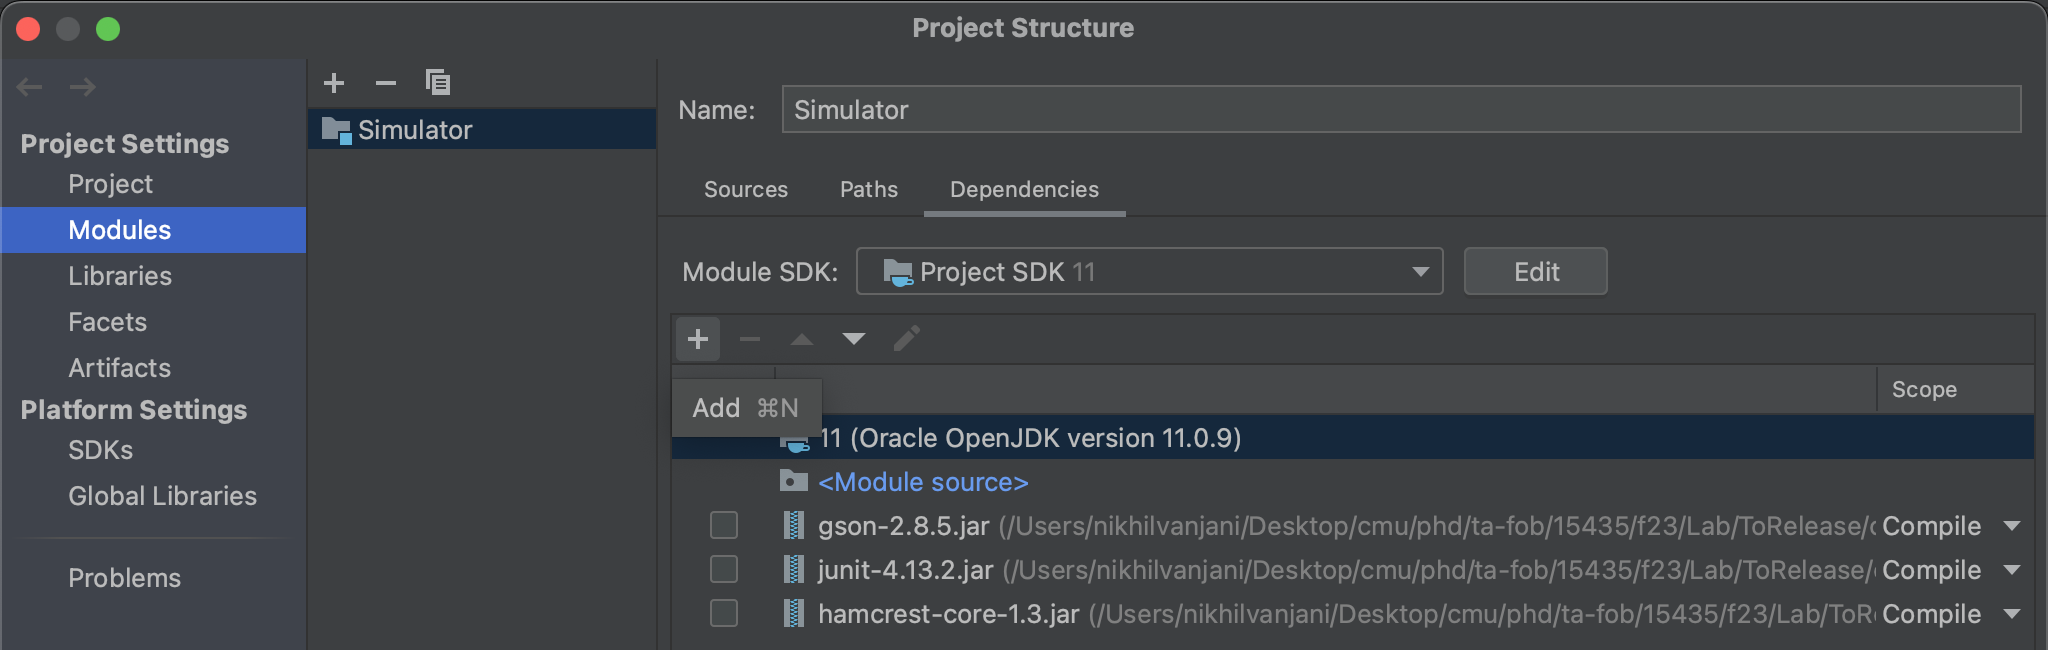
\includegraphics[width=0.7\textwidth]{dependencies.png}
\caption{Adding dependencies in Intellij}
\label{fig:dependencies}
\end{figure}
After these steps are done, you should be able to successfully compile the starter code.

Once the code is compiled, you can run any test in the \texttt{./Test/} directory. For example, to run \texttt{testDrop1} in \texttt{DSTestCases}, go the the \texttt{./Test/DSTestCases.java} file and click the green triangle next to line $12$. If you want to run all the tests in \texttt{DSTestCases}, click the green triangle next to line $10$. If you want to run all the tests for all the checkpoints, click the green triangle next to line $15$ in the \texttt{./Test/RunTests.java} file.
% \bigskip

% Back to the main window, click Add Configurations between the build and run sign, then click + sign on the top left $\rightarrow$ Application, selects main as the main class, then it should be able to run.

% Now you should be able to run the project by clicking the triangle on the top right, and it should output all players' output whether the protocol was broken or not.

\subsection{Shell scripts}
In the {\tt Code} folder, you can find two shell scripts
    {\tt compile.sh} and {\tt run.sh}.
The command {\tt ./compile.sh} compiles all of the code along with the dependencies.
The command {\tt ./run.sh} runs all the test cases that we have provided you.
Alternately, test cases for specific checkpoints can be run as follows.
\begin{itemize}
\item Checkpoint 0: {\tt ./run.sh \ Majority\_Vote\_Adversary}
\item Checkpoint 1: {\tt ./run.sh \ Student\_Player}
\item Checkpoint 2: {\tt ./run.sh \ Dolev\_Strong\_FRound\_Adversary}
\end{itemize}
%\end{document}

\pagebreak

\section{Autograder Integration}

We currently support Gradescope for autograding. There are two options available for integrating the autograder with Gradescope.

\paragraph{Set Up Your Own Autograder}
Our project is compatible with Gradescope, as we utilize JUnit tests in the \texttt{Test} class. To integrate your autograder, follow the instructions provided in the \href{https://gradescope-autograders.readthedocs.io/en/latest/getting_started/#setting-up-your-assignment}{Gradescope Autograder Documentation}  to build your base image and upload it to Gradescope.

Specifically, you will need to create two files
\begin{itemize}
    \item
           \texttt{setup.sh} This file instructs the autograder to install the necessary dependencies for the project.
    \item
          \texttt{run\_autograder}  This file guides the autograder to copy the students' code into the project, compile it, and execute the tests. 
\end{itemize}

Details could be fined in the link above.

\paragraph{Modify Our Autograder}
If you prefer not to build your autograder from scratch, you can contact Junxi Song for access to our autograder configuration, including our test cases. Although the file hierarchy differs slightly from the open-source version, it remains fully functional.


%\end{document}


\end{document}
